\section{控制算法}

本文基于\cite{plestanNewMethodologiesAdaptive2010}提出了一种新的自适应滑膜控制算法来解决上面提出的问题。系统总的控制框图如下:

\begin{figure}[H]
    \centering
    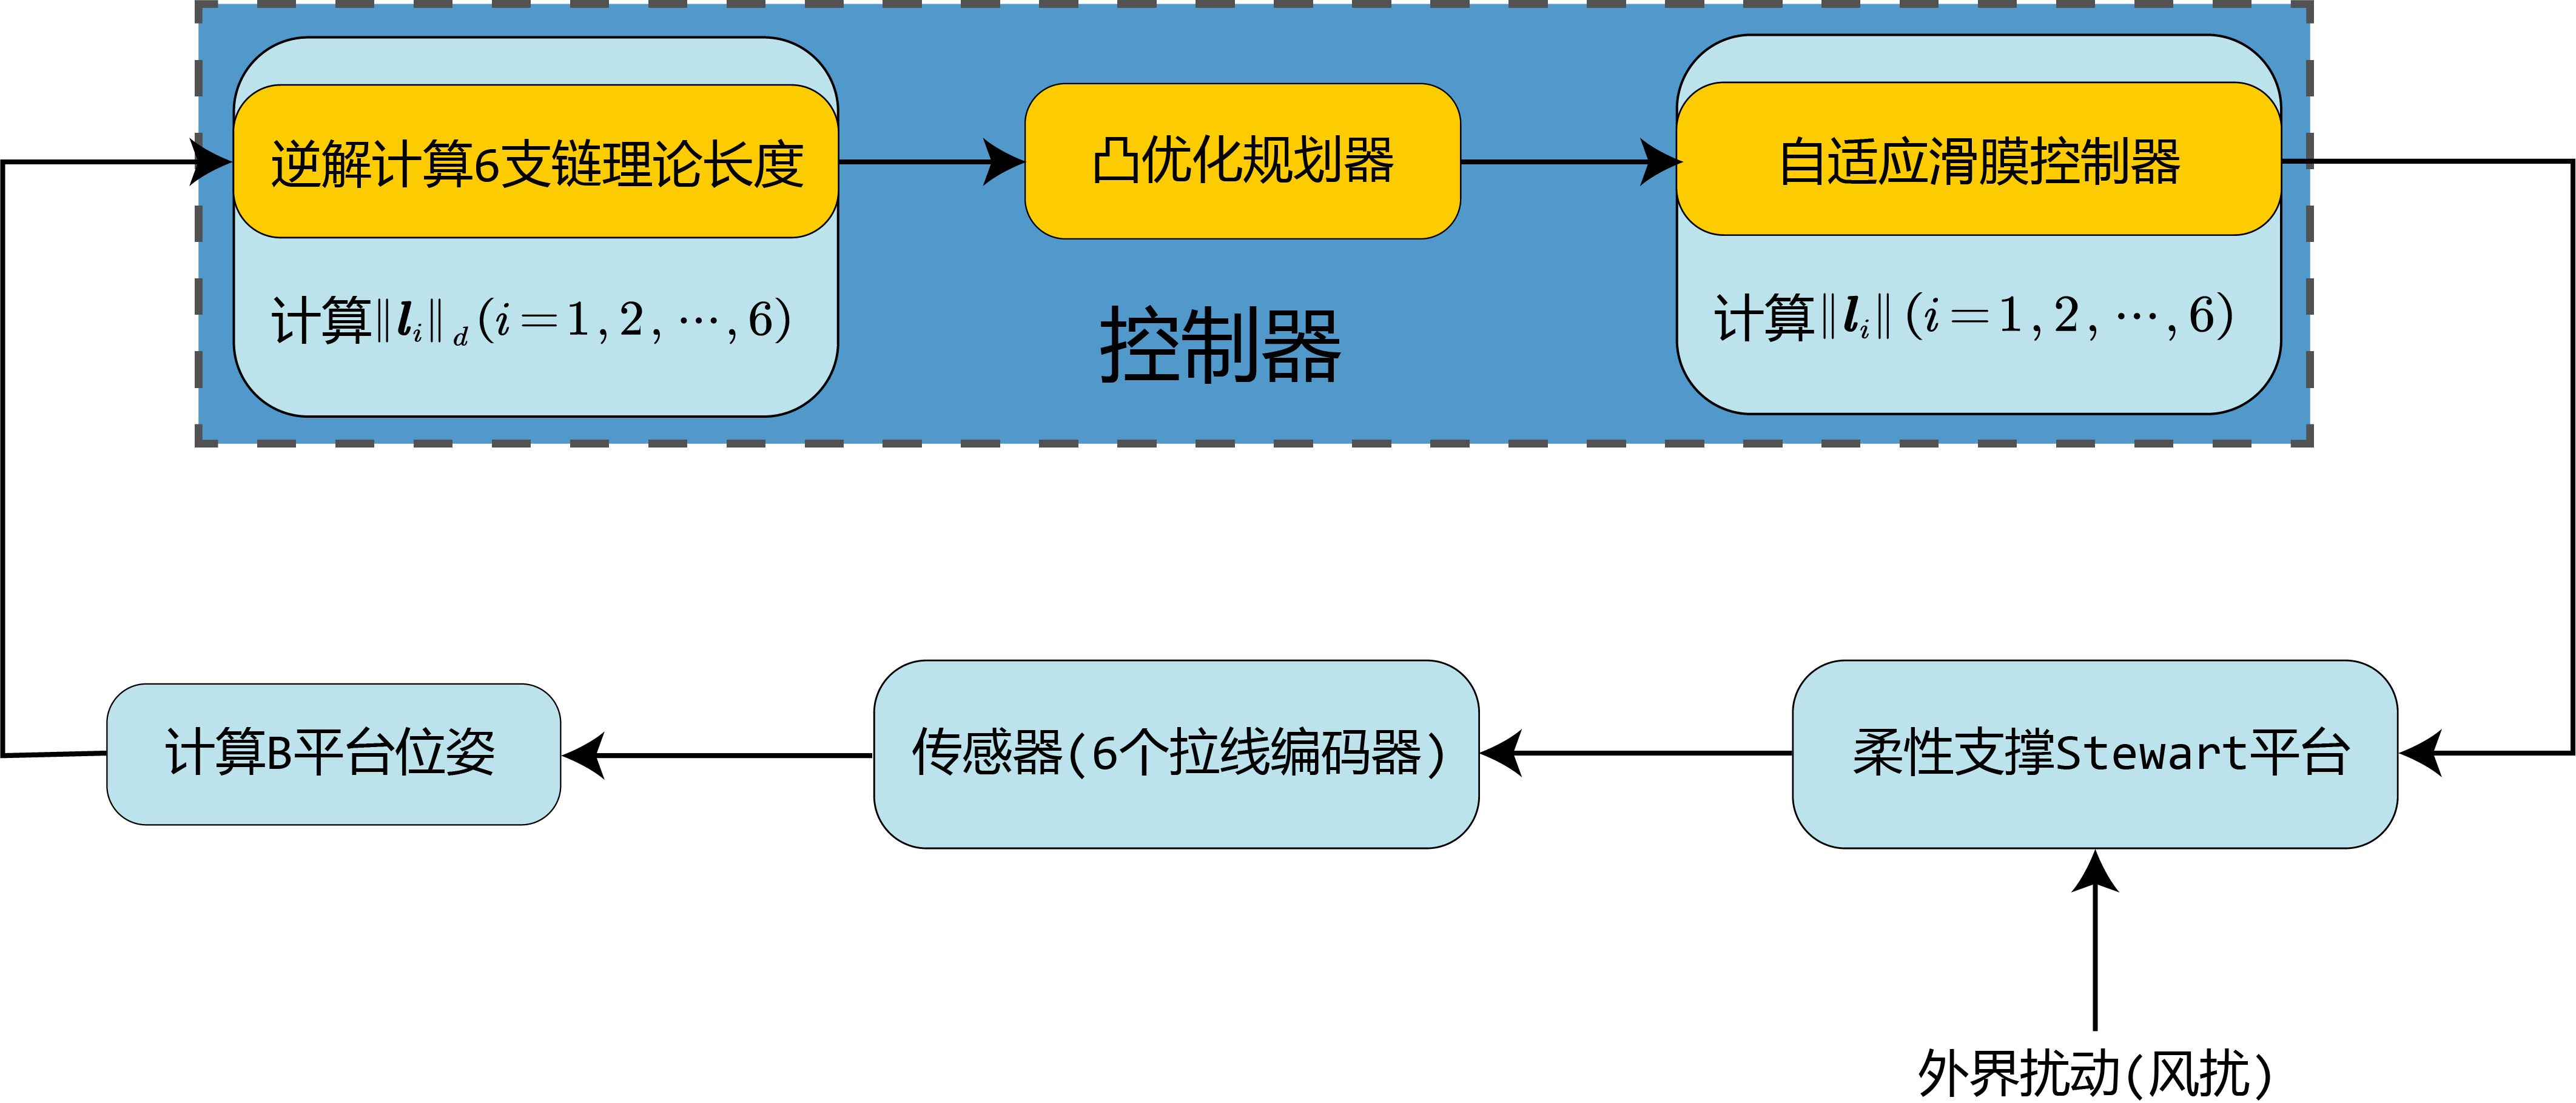
\includegraphics[width=0.6\textwidth]{./imgs/control_model.png}
    \caption{控制框图}
    \label{fig:control_model}
\end{figure}

如图\ref{fig:control_model}所示,控制器由三部分组成:第一级是运动学逆解,用于根据B平台位姿计算出理论上的6条支链长度;第二级是设计的一个凸优化轨迹规划器,用于限制支链运动的最大速度和加速度,保证机构安全;第三级是提出的自适应滑膜控制器,用于自适应地控制输出的实际轴长,减小误差和支链运动带来的影响;

将控制对象抽象为式子(\ref{eqn:sys_model})描述的微分方程,提出下面的控制算法。

\begin{equation}
    \dot{x}=f\left( x \right) +g\left( x \right) u
    \label{eqn:sys_model}
\end{equation}

其中$x\in R^n$是系统的状态变量,$f(x)$和g$(x)$是在$x$定义域内有界的。假定控制的滑膜变量为$\sigma(x,t)$,目的是使得$\sigma=0$。

根据系统方程(\ref{eqn:sys_model}),有

\begin{equation}
    \begin{array}{c}
        \dot{\sigma}=\frac{\partial \sigma}{\partial x}\dot{x}+\frac{\partial \sigma}{\partial t}\\
        =\underset{\varPsi \left( x,t \right)}{\underbrace{\frac{\partial \sigma}{\partial x}f\left( x \right) +\frac{\partial \sigma}{\partial t}}}+\underset{\varGamma \left( x,t \right)}{\underbrace{\frac{\partial \sigma}{\partial x}g\left( x \right) u}}\\
    \end{array}
\end{equation}

根据假设,系统满足:
\begin{equation}
    \left| \varPsi \right|\le \varPsi _M, 0<\varGamma _m\le \varGamma \le \varGamma _M
    \label{eqn:sys_constrain}
\end{equation}

提出自适应滑膜控制器,满足:

\begin{equation}
    \begin{array}{c}
        u=-K\tanh \left( \sigma \left( x,t \right) \right)\\
        \dot{K}=\begin{cases}
        \bar{K}\left| \sigma \left( x,t \right) \right|\mathrm{sign}\left( \left| \sigma \left( x,t \right) \right|-\varepsilon \right)\\
        \mu\\
    \end{cases}\qquad \begin{array}{c}
        \mathrm{if}\quad K>\mu\\
        \mathrm{if}\quad K\le \mu\\
    \end{array}\\
        \bar{K}=\bar{K}_0\exp \left( C_e\left| \sigma \left( x,t \right) \right| \right) , \varepsilon =T_eK\\
    \end{array}
    \label{eqn:controller}
\end{equation}

其中$K\left( 0 \right) >0,C_e>0,\bar{K}_0>0,T_e >0,\mu >0$且$\mu$很小。那么,可以证明,这样的控制器有下面2个特点。

\begin{lemma}
    K存在上界
    \label{lemma1}
\end{lemma}

\begin{figure}[H]
    \centering
    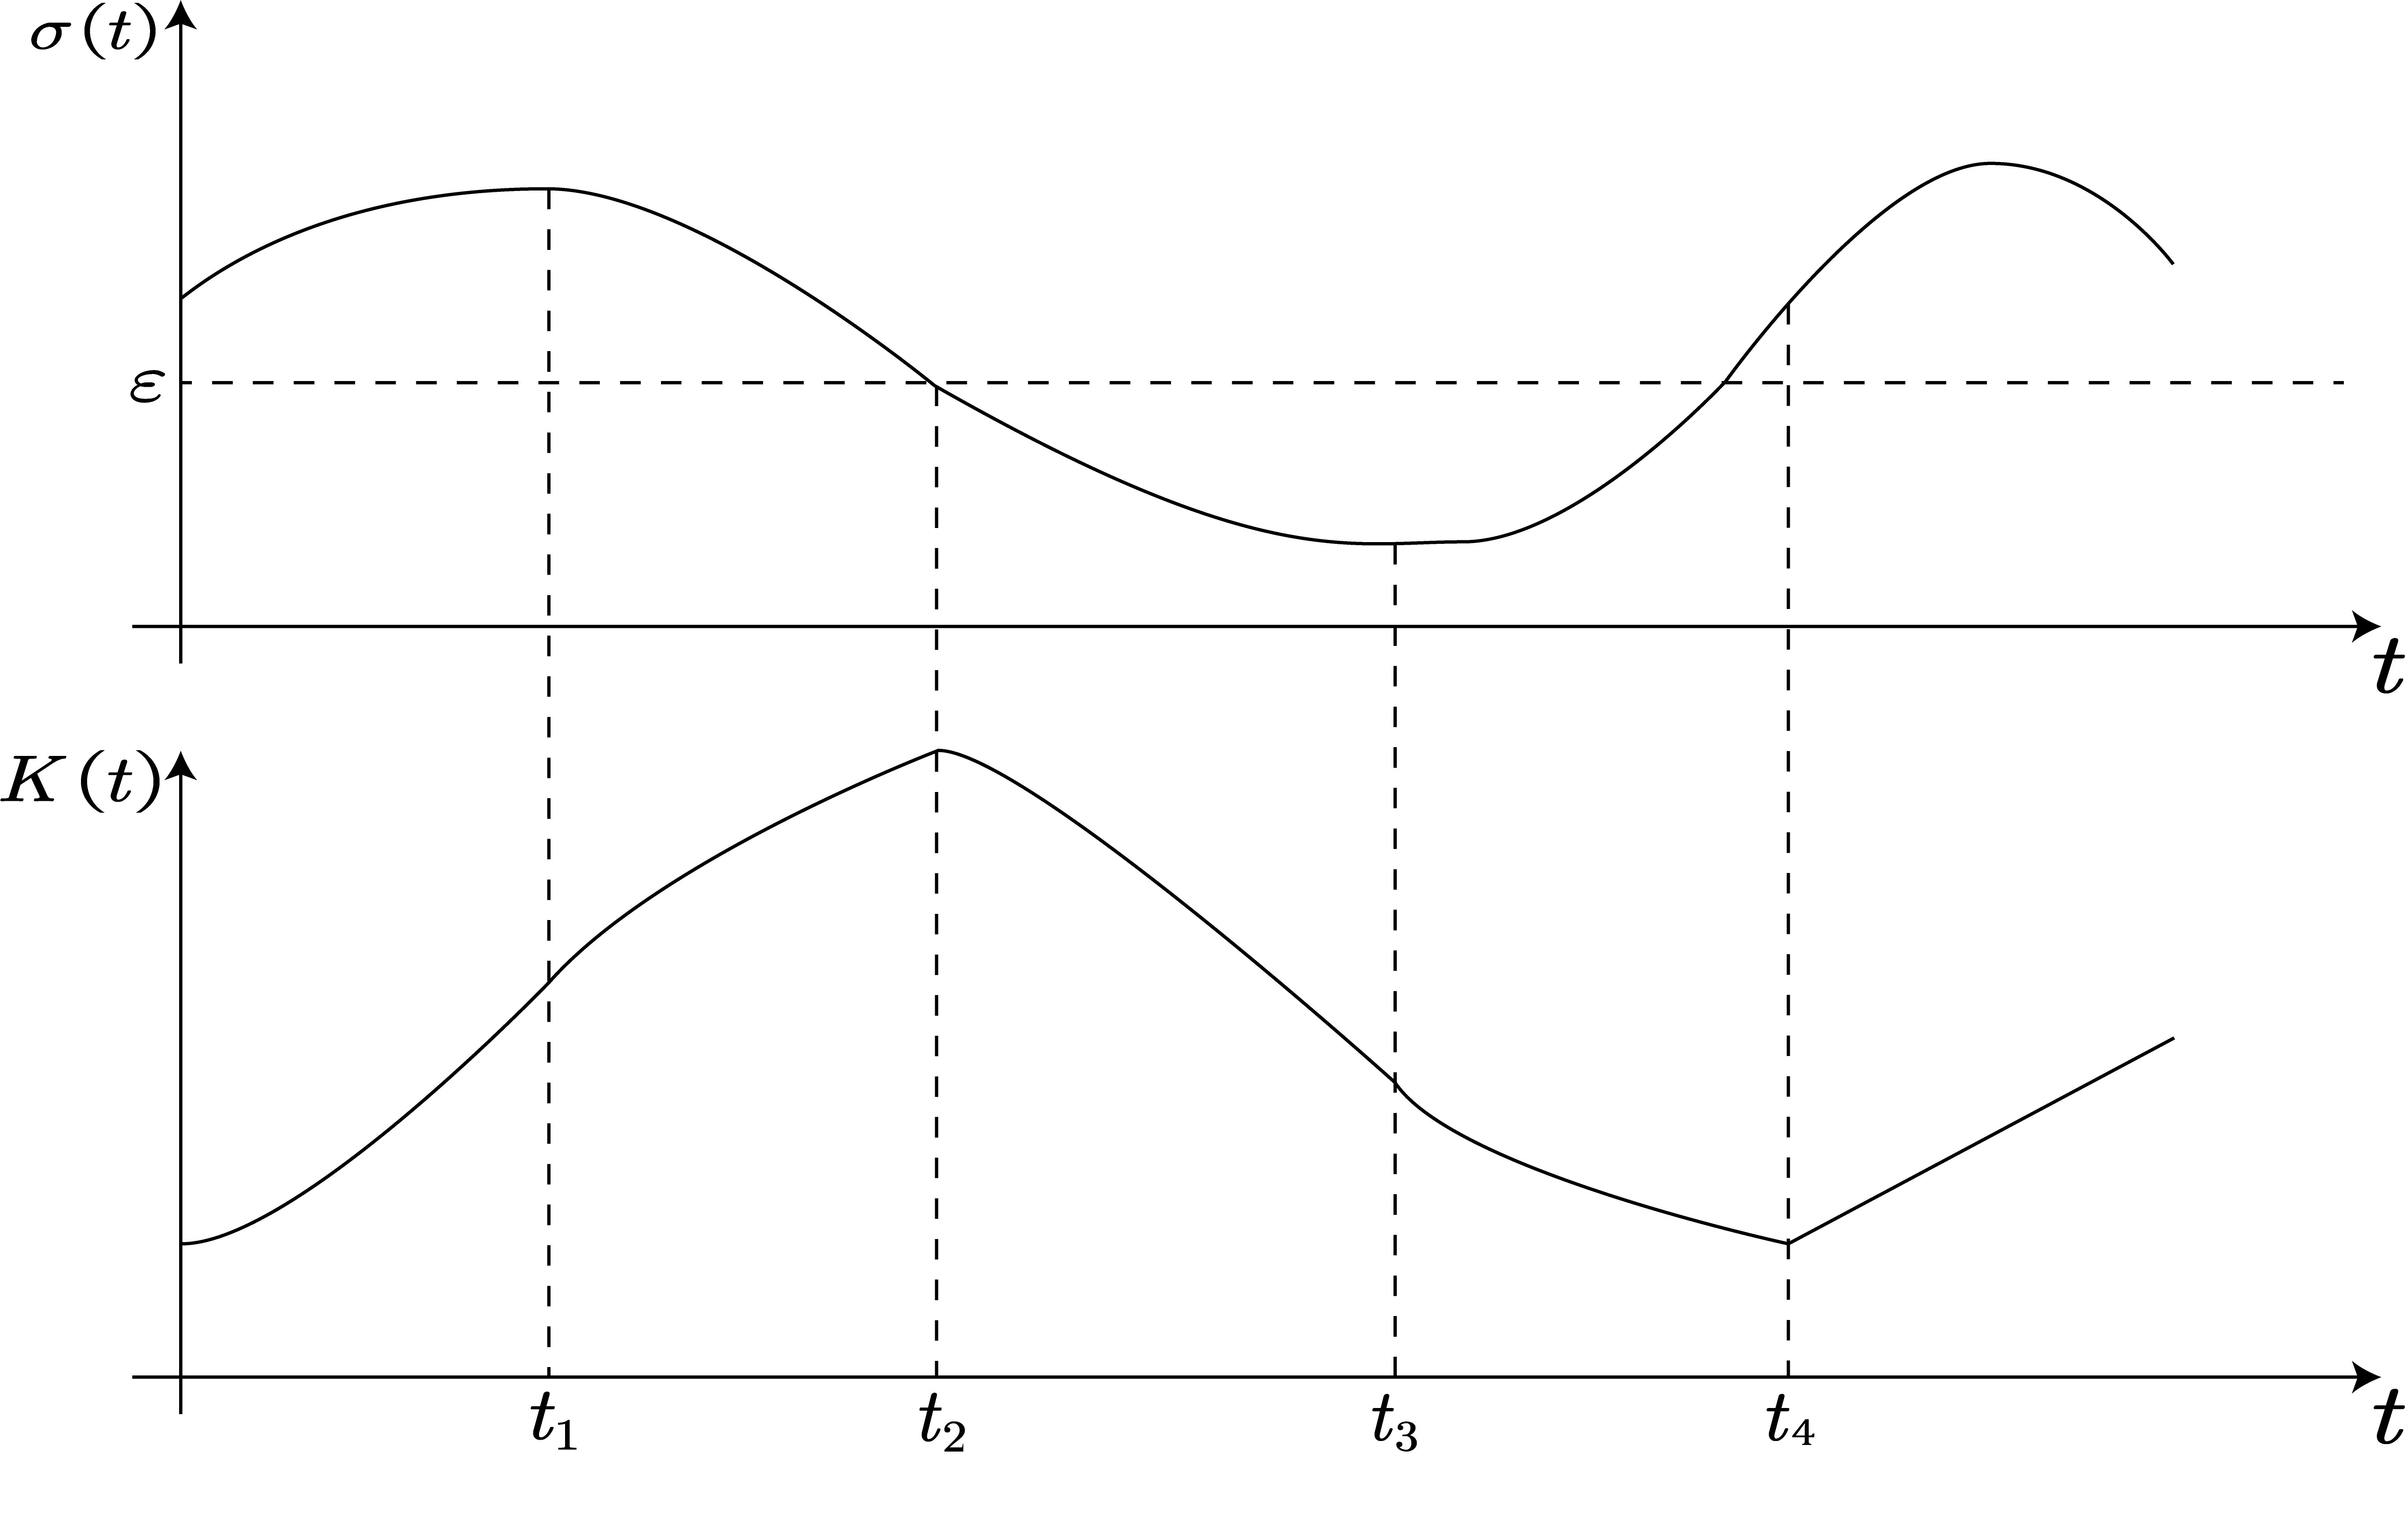
\includegraphics[width=0.6\textwidth]{imgs/math_proof_1.png}
    \caption{一个调节周期内$\sigma$和$K$的变化曲线}
    \label{fig:math_proof_1}
\end{figure}

假定一开始$K>\mu$,$\left| \sigma \left( x,t \right) \right|>\varepsilon$,那么此时K开始增长,且满足增长速率:

\begin{equation}
    \begin{array}{c}
        \dot{K}=\bar{K}_0\exp \left( C_e\left| \sigma \right| \right), \left| \sigma \right|\ge \underset{K_c>0}{\underbrace{\bar{K}T_e}}K\\
        \Rightarrow K\ge \exp \left( K_ct+c \right)\\
    \end{array}
    \label{eqn:l1_Kinit}
\end{equation}

这表明$K$的数值呈指数上升。从而K会一直增加,直到一个$t_1$时刻,此时$u$足够大使得滑膜变量$\sigma$开始减小,即式子(\ref{eqn:l1_sigma_decrease})所示。

\begin{equation}
    \begin{array}{c}
        \dot{\sigma}=\varPsi \left( x,t \right) +\varGamma \left( x,t \right) u\\
        \left| \varPsi \right|\le \varPsi _M, 0<\varGamma _m<\varGamma <\varGamma _M\\
        \Rightarrow \dot{\sigma}\le \varPsi _M+\varGamma _mu, u<0\\
        \Rightarrow \dot{\sigma}<0\quad \mathrm{if}\quad \left| u \right|>\frac{\varPsi _M}{\varGamma _m}\\
    \end{array}
    \label{eqn:l1_sigma_decrease}
\end{equation}

注意到这里$u$增长是指数形式的,从而这里的$t_1$不会太大,基本上是对数时间达到该点。

在此之后K继续增大,直到$\sigma$再次下降到$\varepsilon$,此时K在$t_2$时刻达到最大。注意到从$t_1$到$t_2$过程中,输出$u$相比从开始到$t_1$的阶段更大,因此对我们的系统(\ref{eqn:sys_model})而言,其滑膜变量减小速度比前一段更快,即表明$\left\| t_2-t_1 \right\| \le \left\| t_1 \right\| $,从而这里的K最大值是有限的。继续这个进程,K开始减小,直到$t_3$时刻,K太小以至于无法抵消外界扰动(也就是使得$\sigma$斜率再次为0)。再进一步此时K保持减小,直到误差增大到初始时刻的情况,达到时刻$t_4$,回到一开始的起点。

由于$t_i$时刻是有限的,因此K增加的范围也是有限的。在上述的整个过程中,$t_2$处取得有限的最大值,这表明K存在上界。

\begin{lemma}
    对上面的非线性系统和控制方法,存在有限的时间$t_F>0$使得实际滑模面在所有$t>t_F$的时候成立,即:
\begin{eqnarray}
    \begin{array}{c}
        \left| \sigma \left( x,t \right) \right|<\delta , \forall t\ge t_F\\
        \delta =\ln \left( \exp \left( \sigma _0 \right) +\frac{1}{2\varGamma _m\bar{K}_0}\left( \frac{\varPsi _M}{T_eK\left( 0 \right)}-\varGamma _mK\left( 0 \right) \right) ^2 \right)\\
        t_F=\frac{2\mathrm{arcsech} \left( \sqrt{\frac{-2a}{{\dot{\sigma}_0}^2-2a\exp \left( \sigma _0 \right)}} \right)}{\sqrt{{\dot{\sigma}_0}^2-2a\exp \left( \sigma _0 \right)}}\\
        \sigma _0=\varepsilon ^+\ge \varepsilon =T_eK\left( 0 \right) ,\dot{\sigma}_0=\varPsi _M-\varGamma _m\varepsilon ^+K\left( 0 \right)\\
        a=-\varGamma _m\bar{K}_0\left( \varepsilon ^+ \right) ^2\\
    \end{array}
    \label{eqn:l2_actual_sliding_model}
\end{eqnarray}
\label{lemma2}
\end{lemma}

考虑李雅普诺夫函数,有:

\begin{eqnarray}
    V=\frac{1}{2}\sigma ^2+\frac{1}{2\gamma}\left( K-K^* \right) ^2
    \label{enq:l2_lyaponiv}
\end{eqnarray}

其中$K^*$是K的上界。对V时间微分有式子(\ref{eqn:l2_dV}):

\begin{eqnarray}
    \begin{array}{c}
        \dot{V}=\sigma \left( \varPsi -\varGamma K\tanh \left( \sigma \right) \right) +\frac{1}{\gamma}\left( K-K^* \right) \bar{K}\left| \sigma \right|\mathrm{sign}\left( \left| \sigma \right|-\varepsilon \right)\\
        \le \varPsi _M\left| \sigma \right|-\varGamma _mK\left| \sigma \right|+\frac{1}{\gamma}\left( K-K^* \right) \bar{K}\left| \sigma \right|\mathrm{sign}\left( \left| \sigma \right|-\varepsilon \right)\\
        =\varPsi _M\left| \sigma \right|-\varGamma _mK\left| \sigma \right|+\underset{\text{构造项}}{\underbrace{\varGamma _mK^*\left| \sigma \right|-\varGamma _mK^*\left| \sigma \right|}}+\frac{1}{\gamma}\left( K-K^* \right) \bar{K}\left| \sigma \right|\mathrm{sign}\left( \left| \sigma \right|-\varepsilon \right)\\
        =\left( \varPsi _M-\varGamma _mK^* \right) \left| \sigma \right|+\left( K-K^* \right) \left( -\varGamma _m\left| \sigma \right|+\frac{1}{\gamma}\bar{K}\left| \sigma \right|\mathrm{sign}\left( \left| \sigma \right|-\varepsilon \right) \right)\\
    \end{array}
    \label{eqn:l2_dV}
\end{eqnarray}

进一步添加构造项$\beta_{K}>0$有:

$$\begin{array}{c}
	\dot{V}\leq \left( \varPsi _M-\varGamma _mK^* \right) \left| \sigma \right|+\left( K-K^* \right) \left( -\varGamma _m\left| \sigma \right|+\frac{1}{\gamma}\bar{K}\left| \sigma \right|\mathrm{sign}\left( \left| \sigma \right|-\varepsilon \right) \right)\\
	+\beta _K\left| K-K^* \right|-\beta _K\left| K-K^* \right|\\
\end{array}$$

根据引理\ref{lemma1},K存在上界,则有式子(\ref{eqn:l2_Kg0})

\begin{equation}
    K\left( t \right) -K^*<0,\forall t>0
    \label{eqn:l2_Kg0}
\end{equation}

从而有式子(\ref{eqn:l2_dVl0})

\begin{equation}
    \begin{array}{c}
        \dot{V}\leq -\underset{\beta _{\sigma}>0}{\underbrace{\left( -\varPsi _M+\varGamma _mK^* \right) }}\left| \sigma \right|-\beta _K\left| K-K^* \right|\\
        -\underset{\xi}{\underbrace{\left| \underset{<0}{\underbrace{K-K^*}} \right|\left( -\varGamma _m\left| \sigma \right|+\frac{1}{\gamma}\bar{K}\left| \sigma \right|\mathrm{sign}\left( \left| \sigma \right|-\varepsilon \right) -\beta _K \right) }}\\
    \end{array}
    \label{eqn:l2_dVl0}
\end{equation}

这意味着式子(\ref{eqn:l2_dVl0_1}):

\begin{equation}
    \begin{array}{c}
        \dot{V}\leq -\beta _{\sigma}\left| \sigma \right|-\beta _K\left| K-K^* \right|-\xi\\
        =-\beta _{\sigma}\sqrt{2}\frac{\left| \sigma \right|}{\sqrt{2}}-\beta _K\sqrt{2\gamma}\frac{\left| K-K^* \right|}{\sqrt{2\gamma}}-\xi\\
        \dot{V} \le -\min \left\{ \beta _{\sigma}\sqrt{2}, \beta _K\sqrt{2\gamma} \right\} \left( \frac{\left| \sigma \right|}{\sqrt{2}}+\frac{\left| K-K^* \right|}{\sqrt{2\gamma}} \right) -\xi\\
        \le -\beta V^{1/2}-\xi, \quad \beta =\min \left\{ \beta _{\sigma}\sqrt{2}, \beta _K\sqrt{2\gamma} \right\}\\
    \end{array}
    \label{eqn:l2_dVl0_1}
\end{equation}

现在分析$\xi$的情况。

\textbf{Case1: $\left| \sigma \right|>\varepsilon$}

由于$\left| \sigma \right|>\varepsilon$,此时有式子(\ref{eqn:l2_xi_1})

\begin{equation}
    \begin{array}{c}
        \xi =-\varGamma _m\left| \sigma \right|+\frac{1}{\gamma}\bar{K}_0\exp \left( \left| \sigma \right| \right) \left| \sigma \right|\mathrm{sign}\left( \left| \sigma \right|-\varepsilon \right) -\beta _K>0\\
        \Longleftrightarrow \gamma <\frac{\bar{K}_0\exp \left( \left| \sigma \right| \right) \left| \sigma \right|}{\varGamma _m\left| \sigma \right|+\beta _K}\\
    \end{array}
    \label{eqn:l2_xi_1}
\end{equation}

注意到右边函数是增函数,因此取:

\begin{equation}
    \gamma <\frac{\bar{K}_0\exp \left( \varepsilon \right) \varepsilon}{\varGamma _m\varepsilon +\beta _K}
\end{equation}

对于给定的$\varepsilon$,存在这样的$\gamma$。
此时有式子(\ref{eqn:l2_dV_c1})

\begin{equation}
    \dot{V}\le -\beta V^{1/2}-\xi \le -\beta V^{1/2}
    \label{eqn:l2_dV_c1}
\end{equation}

根据李雅普诺夫收敛的性质,这表明在任何$\left| \sigma \right|>\varepsilon$的条件下,控制对象在有限时间内收敛。

\textbf{Case2: $\left| \sigma \right|<\varepsilon$}

此时$\xi$可能为负,这意味着李雅普诺夫的思路不能完全成功。但可以注意到,一旦$\left| \sigma \right|>\varepsilon$,立马问题就解决了。因此我们需要考虑的问题从最坏情形来分析,实际上是在考虑下面的情况:

在$\left| \sigma \right|<\varepsilon$切换到$\left| \sigma \right|>\varepsilon$之后,V从Case1情形,即$\left| \sigma \right|>\varepsilon$收敛回$\left| \sigma \right|<\varepsilon$所需要花费的成本。
Case1中使用李雅普诺夫稳定性分析证明了一定是会收敛回来的,而且其耗费的时间是对数的。因此问题化简为考虑最坏情形的误差成本——分析状态切换需要的时间代价和精度问题。

记$\sigma _0=\sigma \left( 0 \right) =\varepsilon ^+>\varepsilon$,$K_0=\mathcal{K} \left( 0 \right) =K\left( 0 \right)$。不失一般性,可以假设$\sigma_0>0$,否则其会一直增长。考虑最坏情形,即式子(\ref{eqn:l2_worst_case}):

\begin{equation}
    \begin{array}{c}
        \dot{\sigma}=\underset{P_m}{\underbrace{\varPsi _M}}-\underset{T_m}{\underbrace{\varGamma _m\varepsilon ^+}}K\\
        \dot{K}=\bar{K}_0\sigma \exp \left( \sigma \right) \ge \underset{K_m}{\underbrace{\bar{K}_0\varepsilon ^+}}\exp \left( \sigma \right)\\
        \sigma \left( 0 \right) =\varepsilon ^+>T_eK\left( 0 \right)\\
    \end{array}
    \label{eqn:l2_worst_case}
\end{equation}

这里的最坏情形意思是放任$\sigma$增大,此时偏离滑模面的误差最大的情况。

注意这里$C_e>0$,对$\sigma$而言,实际上代表着一个时间上的放缩,因此可以假设$C_e=1$。

从而问题可以转化为求解方程(\ref{eqn:l2_dsigma}):

\begin{equation}
    \begin{array}{c}
        \ddot{\sigma}=\underset{a}{\underbrace{-T_mK_m}}\exp \left( \sigma \right)\\
        \sigma \left( 0 \right) =\varepsilon ^+>T_eK\left( 0 \right)\\
    \end{array}
    \label{eqn:l2_dsigma}
\end{equation}

通过令$\sigma(t)=e^{f(t)}$进行变换,可以得到式子(\ref{eqn:l2_dsigma})的解为式子(\ref{eqn:l2_sigma}):

\begin{equation}
    \sigma \left( t \right) =\log \left( \frac{c_1\left( \tanh ^2\left( \frac{1}{2}\sqrt{c_1(c_2+t)^2} \right) -1 \right)}{2a} \right) 
    \label{eqn:l2_sigma}
\end{equation}

其中$c_1,c_2$为待定项,根据$\sigma$的初值条件确定。

带入原问题的初值条件,可以将$\sigma$表示为式子(\ref{eqn:l2_sigma_real}):

\begin{equation}
    \begin{array}{c}
        \sigma \left( t \right) =\ln \left( \frac{-s}{2a}\left( 1+\tan \left( \frac{1}{2}\left( it\sqrt{s}-2i\tanh ^{-1}\left( \frac{\dot{\sigma}_0}{\sqrt{s}} \right) \right) \right) \right) \right)\\
        s={\dot{\sigma}_0}^2-2a\exp \left( \sigma _0 \right) >0, a<0\\
    \end{array}
    \label{eqn:l2_sigma_real}
\end{equation}

考虑其在时间上的最大值,直接微分并求零点得到最大值满足式子(\ref{eqn:l2_sigma_max}):

\begin{equation}
    \begin{array}{c}
        \sigma _{\max}=\ln \left( \exp \left( \sigma _0 \right) -\frac{{\dot{\sigma}_0}^2}{2a} \right) =\ln \left( \exp \left( \sigma _0 \right) +\frac{{\dot{\sigma}_0}^2}{2\varGamma _m\bar{K}_0\left( \varepsilon ^+ \right) ^2} \right)\\
        \sigma _0=\varepsilon ^+, \dot{\sigma}_0=\varPsi _M-\varGamma _m\varepsilon ^+K\left( 0 \right)\\
        t_{\max}=\frac{2\mathrm{arcsech} \left( \sqrt{\frac{-2a}{{\dot{\sigma}_0}^2-2a\exp \left( \sigma _0 \right)}} \right)}{\sqrt{{\dot{\sigma}_0}^2-2a\exp \left( \sigma _0 \right)}}, a=-\varGamma _m\bar{K}_0\left( \varepsilon ^+ \right) ^2\\
    \end{array}
    \label{eqn:l2_sigma_max}
\end{equation}

从幅值收敛情况来看,整体的极限情况偏差距离是有限的,且注意到$\varepsilon ^+\ge \varepsilon =T_eK\left( 0 \right)$,这表明式子(\ref{eqn:l2_sigma_max_1}):

\begin{equation}
    \begin{array}{c}
        \sigma _{\max}=\ln \left( \exp \left( \sigma _0 \right) +\frac{1}{2\varGamma _m\bar{K}_0}\left( \underset{L}{\underbrace{\frac{\varPsi _M}{\varepsilon ^+}-\varGamma _mK\left( 0 \right) }} \right) ^2 \right)\\
        \le \ln \left( \exp \left( \sigma _0 \right) +\frac{1}{2\varGamma _m\bar{K}_0}\left( \frac{\varPsi _M}{T_eK\left( 0 \right)}-\varGamma _mK\left( 0 \right) \right) ^2 \right)\\
        \sigma _0=\varepsilon ^+\ge \varepsilon =T_eK\left( 0 \right) , L=\frac{\dot{\sigma}_0}{\varepsilon ^+}>0\\
    \end{array}
    \label{eqn:l2_sigma_max_1}
\end{equation}

注意到$\dot{\sigma}_0>0$,这使得$L>0$。从而可以发现K越大,收敛前的超差越小。

相比Plestan所提出模型最坏情况下的超差函数,这里的函数是对数的,在大误差的时候收敛情况更优。

Plestan论文中的超差函数\cite{plestanNewMethodologiesAdaptive2010}:

\begin{equation}
    \begin{aligned}
        \sigma (t)=&\sigma _0\cos \left( \sqrt{\bar{K}\Gamma _m}t \right) +\frac{\Psi _M-K_0\cdot \Gamma _m}{\sqrt{\bar{K}\Gamma _m}}\cdot \sin \left( \sqrt{\bar{K}\Gamma _mt} \right)\\
        K(t)=&\sigma _0\sqrt{\frac{\bar{K}}{\Gamma _m}}\sin \left( \sqrt{\bar{K}\Gamma _mt} \right) +\left( K_0-\frac{\Psi _M}{\Gamma _m} \right)\\
        &\times \cos \left( \sqrt{\bar{K}\Gamma _mt} \right) +\frac{\Psi _M}{\Gamma _m}\\
    \end{aligned}
\end{equation}

在$\sigma _0=\varepsilon ^+\rightarrow \varepsilon$时,最大的误差满足

\begin{equation}
    \begin{array}{c}
        \sigma _M=\sqrt{\sigma _{0}^{2}+\frac{\left( \Psi _M-K_0\cdot \Gamma _m \right) ^2}{\bar{K}\Gamma _m}}\\
        \le \sqrt{\varepsilon ^2+\frac{\Psi _{M}^{2}}{\bar{K}\Gamma _m}}\\
    \end{array}
\end{equation}

根据式子(\ref{eqn:l2_sigma_max_1}),这意味着$\sigma$可以在有限时间内以对数的超差收敛到Case1的情况,满足Levant提出的的真实滑模面的定义\cite{levantSlidingOrderSliding1993}。

总的来说,本文提出的自适应滑膜控制律和Plestan所提出的控制律主要有下面2点差别:
\begin{enumerate}
    \item 根据引理\ref{lemma2},选用了指数形式的更新K收敛速度项,使得在出现超出滑模面的情况下,可以以对数形式收敛回滑模面
    \item 目标输出函数选用的是光滑的tanh,相比sign函数减少了波动,保证了输出函数的连续性,在实际应用上更优
\end{enumerate}
\FloatBarrier